\lab{Application}{Nearest Neighbor Search}{Nearest Neighbor Search}
\label{Ch:NNS}

\objective{Teach about branch and bound and the curse of dimensionality using the nearest neighbor search problem.}

\section*{The Nearest Neighbor Search Problem}

You move into a city that has several post offices.
You want to know which one is the closest.
This problem is  known as the nearest neighbor search problem or the post-office problem.
The general problem is to find the closest of a set of points to any new point.

This has many applications which include computer vision, pattern recognition, internet marketing and data compression.

The naive way to solve this problem is to check the distance of all the data against the point.

\begin{problem}
Write a function that solves the nearest neighbor search problem by exhaustively checking all the distances.
The function should take in the set of points that is the data and a single point.
The output should be the distance to the closest data point and the index of that point.
Your function should be able to take in data in an arbitrary dimension.
\end{problem}

The complexity of this algorithm is $O(kn)$.
Where  is the $k$ number of dimensions and $n$ is the number of data points.

\section*{K-D Trees}

A faster way to solve this problem is to build a k-d tree and search the k-d tree for the nearest neighbor. 

A k-d tree is a binary tree where the nodes to the left of parent node have a lower value in the i-th dimension and the nodes to the right of the parent node have a greater value in the i-th dimension.
Which dimension you split the nodes alternates at different levels.
In the $3$ dimensional case the root node is divided in the $x$ dimension, children in the $y$ dimension, grandchildren in the $z$ dimension, and the great-grandchildren in the $x$ dimension and so on.
Each node stores its location, left child and right child.
This requires sorting at each level so the complexity is $O(n log^2(n))$, but we only need to build the k-d tree once and after that we can query it as many times as we want.

Included is a function that takes in a set of data and builds k-d tree.
The leaf nodes' children are  python's ``None" object.

The search of the tree is done recursively.
Our search function will accept a parent node on which to search, a search point to which we want to find the nearest neighbor, the current best point, the current best distance, and a dimension $i$.
The search function should return the best point and best distance currently held in the algorithm.
We start the algorithm on the root node of the tree using it's point and distance to the search point as the best point and best distance, and start with $0$ as the first dimension.


For each recursive step, we first check if the euclidean distance between the parent node's point to the search point is less than the current best.
If so, we update it the best distance and best point to match the parent node.


We then compare the values in the $i$-th dimension of the search point and the parent's point.
If the search point's value is less than that of the parent node's point we recursively call the search function again on the left child of the parent node on the dimension $i+1$, flipping the dimension to $0$ if necessary, and set best point and best distance to it's output.
Then we have to check if the hypersphere around the point with radius being the current best distance crosses the dividing hyperplane created by the parent.
In code we accomplish this by adding the best distance to the point's value in the $i$-th dimension.
If this sum is greater than the parent's point value in the i-th dimension, we then search additionally the right child of the parent (using the dimension $i+1$) and update the best point and best distance to the output.


If the point's value was less than the parent's in th i-th dimension, we apply the last two steps mirrored to the right and left children.
We first search the right child with the $i+1$-th dimension and set the best point and best distance to the output.
We then check if the search point's value in the $i$-th dimension minus the best distance is less than the parent node's value in the $i$-th dimension. 
If it is, we will also search the left child one the $i+1$-th dimension and set the best point and best distance to the output.

Below the algorithm summarized in pseudo code 

\begin{algorithm}
\begin{algorithmic}[1]
\Procedure{KDSearch}{search\_point,parent\_node,b\_point,b\_distance,i}
    \If { Distance(search\_point,parent\_node.point) $<$ b\_distance }
        \State b\_point = parent\_node.point
        \State b\_distance = Distance from search\_point to parent\_node.point
    \EndIf

    \If{search\_point[i] $<$ parent\_node.point[i]}
        \State b\_point, b\_distance =
            \State KDSearch(search\_point,parent\_node.left\_child,b\_point,b\_distance,i+1)
        \If { search\_point[i] + b\_distance $geq$ parent\_node.point} 
            \State b\_point, b\_distance = 
                \State KDSearch(search\_point,parent\_node.right\_child,b\_point,b\_distance,i+1)
        \EndIf
    \Else
        \State b\_point, b\_distance = 
            \State KDSearch(search\_point,parent\_node.right\_child,b\_point,b\_distance,i+1)
        \If {search\_point[i] + b\_distance $leq$ parent\_node.point} 
            \State b\_point, b\_distance = 
                \State KDSearch(search\_point,parent\_node.left\_child,b\_point,b\_distance,i+1)
        \EndIf
    \EndIf
\EndProcedure
\end{algorithmic}
\caption{Nearest Neighbor}
\label{alg:nearestneighbor}
\end{algorithm}


\begin{problem}
Write a function that solves the nearest neighbor search problem by searching through a k-d tree.
The function should take in k-d tree and a single point.
The output should be the distance to the closest data point and the coordinates of that point. 
\end{problem}

\begin{problem}
Time both the functions you have created with the number of data points being $10,000-100,000$ every multiple of $10,000$ with $4$ dimensions.
Time only the searching of the k-d tree not the building of it.
Plot both times on the same plot.
How do the two algorithms compare?
\end{problem}

\begin{figure}[H]
\includegraphics[scale = .5]{4dTime.pdf}
\caption{Your graph should look like this.
The green line is the naive version and blue line is using a kd-tree.
As you can see the kd-tree is much faster.}
\end{figure}

The complexity of this algorithm is $O(klog(n))$ in optimal time.
Its worst case is $O(k*n^{1-\frac{1}{k}})$ where $k$ is the number of dimensions and $n$ is the number of points in the tree.
The reasons for this are discussed in the next section.

\section*{Curse of Dimensionality}

As you increase the number of dimensions the number of times that you have to go down both branches increases.
You get to the point where you eliminate very few points by using a k-d tree.

\begin{problem}
Time both algorithms for the number of data points being $10,000-100,000$ every multiple of $10,000$ with $20$ dimensions.
Plot both times on the same plot. Now how do the two algorithms compare?
\end{problem}

\begin{figure}[H]
\includegraphics[scale = .5]{20dTime.pdf}
\caption{
Your graph should look like this.
The green line is the naive version and blue line is using a kd-tree.
As you can see the kd-tree is slightly slower than the naive version.}
\end{figure}

\begin{problem}
Time the SciPy built in function for searching a k-d tree (do not time the building of the kd-tree) for the number of dimensions points being $2-50$ with $20,000$ data points.
Plot the time.
What do you notice?
\li{from scipy.spatial import KDTree} will import the built in k-d tree.
Create the tree by \li{tree = KDTree(data)} and search it by \li{tree.query(point)}.

\li{scipy.spatial} includes a \li{cKDTree} object which is implemented in C.
Is it any better?

\end{problem}
\begin{figure}[h!]
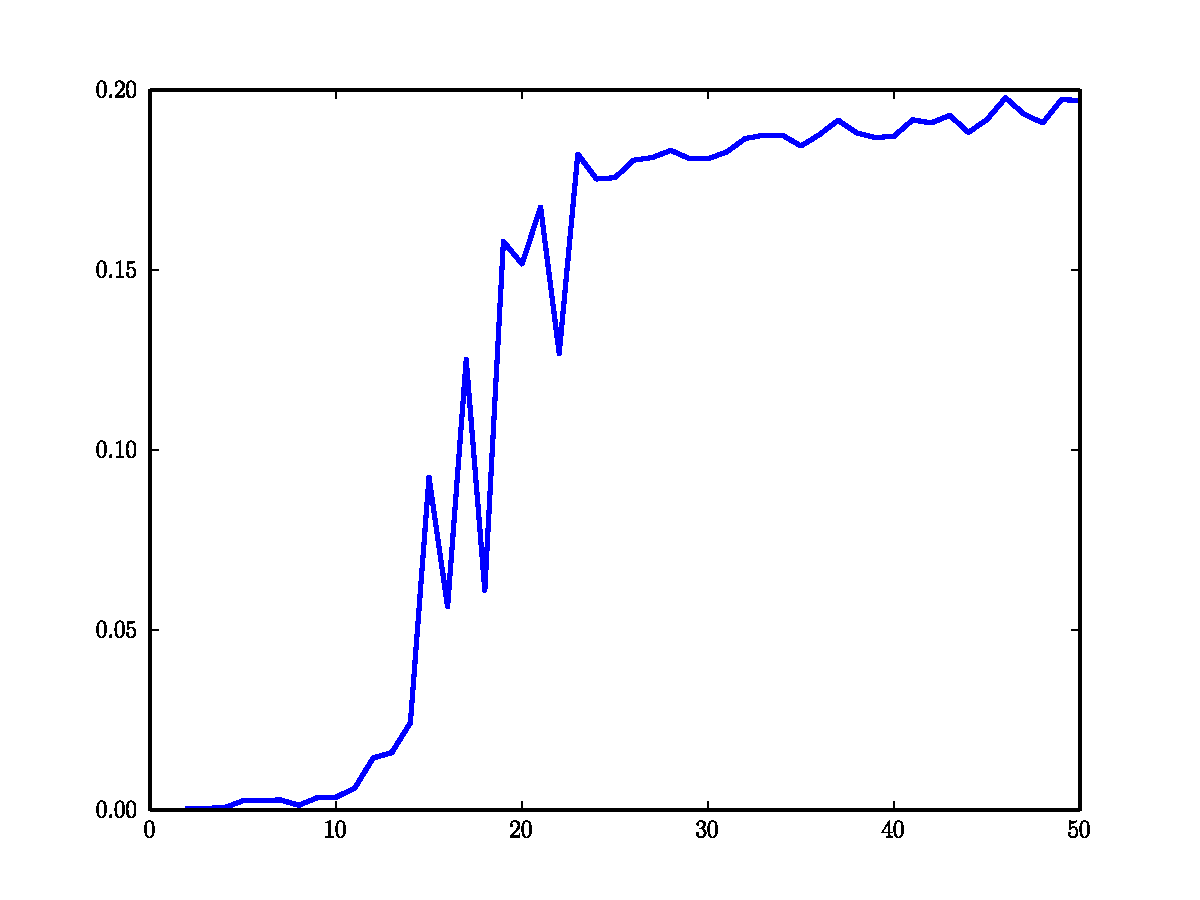
\includegraphics[scale = .5]{curseD.pdf}
\caption{
Your graph should look similar to this.
Around 15 dimensions the time jumps.
At that point using a kd-tree is not more effective than checking all the combinations.}
\end{figure}


